\documentclass[../notebook.tex]{subfiles} 

\linespread{1.2} % line spread
\begin{document}
\begin{center}

\end{center}

\section{ C++ and memory management }
In this lesson, you will learn how C++ manages memory, and you will gain understanding of how memory is managed inside your computer. Understanding these concepts is very important for programmers for several reasons:
\begin{itemize}
  \item Allows you to optimize your program, avoiding to allocate useless memory.
  \item Understand what goes under the hood in dynamic programming languages.
  \item Can avoid security issues.
  \item Learn our first data structure!
\end{itemize}
\subsection{ Process memory } % (fold)
\label{sub:subsection name}
\begin{figure}
  \centering
  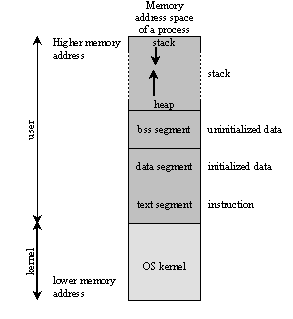
\includegraphics[scale=.88]{mstack.png}
  \caption{ Process memory }
  \label{fig:mstack}
\end{figure}
Every process inside a computer has a certain amount of memory, which is granted to the process by the operative system. Some of that memory will be reserved to keep some information about the process. That memory cannot be accessed, and is reserved to the operative system.  Then, we have that is called the {\bf stack}. Look at Figure \ref{fig:mstack} to get an idea of how process memory looks like:\\
\subsubsection{Stack}
The stack is used in order to keep track of the location where we are inside our process. Imagine that you have a certain number of tasks that you need to do. For every task, we make a post-it, with some information about the task. A task may require you to have to complete a different task before you may be able to solve the previous one, and for every task you need to store some information, relative to the task. How are we going to keep track of all the post-its that we will write? \\
An excellent way to manage this information is to use a pile. For every post-it that we make, we will push it on top our pile. If the task will require some other task to be completed, then we will begin working on that task, and push the relative post-it on top of our pile. Once a task is completed, then we remove the post-it from the top of our pile, and resume working on the task with the previous post it. When, the pile will be empty again, then our program will be over! \\
In computers programs, things work in the same way. Instead of tasks we have functions, and our pile is what we refer to as a stack, an abstract data structure. The information that we need in our process are variables, that we need to keep track of in order to complete our tasks. The post-its are the chunks of memory that we use to store that information inside our process. Lets take a look at an example:
\begin{cppcode}
  int task ( int sum )
  {
    int total = 0;
    for ( int i =0; i < sum; i++ )
      total +=i; 
    return total;
  }

  int main ( int argc, const char * argv[] ) 
  { //  This is the entry point of our program.
    int sum = 5;
    int total = task( sum );
    total    += task( sum ); // += will add to the existing value
    return 0; 
  }
\end{cppcode}
Now, lets take a look at what happens inside our stack when we execute the program. We start with main inside the stack. Inside the space for main, there will be enough space for the variables $sum$, and $total$. On line \emph{13}, the variable sum will take the value 5. Then, the function $task$ will be called. \\
New space will be asked for on the stack, so that we can fit the variables that we have inside $task$. The value of $sum$ will be copied over, and the function $task$ will have its own copy. Likewise, $task$ will have its own version of $total$. These are {\bf local variables}, so they only exist in the scope of the function. You cannot access the local variables of  $main$ from the function $task$. Once the first call to $task$ will be completed, we will copy the value of $total$ to the main function, and the space on the stack that was reserved to $task$ will be erased. Just like in our analogy we used to throw away post-its once they were completed. This is how the memory stack works! \\
\subsubsection{Heap}
There is one more complication to how memory management works. Imagine, we are in the middle of one of our functions/tasks. All of a student, we discover that we need more memory than we thought before. Where do we get the memory from? We cannot change the size of memory that we have on the stack, yet we need more memory. This is where dynamic memory comes in. If we do not know the amount of memory that we are going to use for a certain task, then we are going to use something called the {\bf heap}. The heap is another memory segment in the process memory. It is used to allocate dynamic memory. You can allocate and free memory on the heap as you wish, without many limitations. In order to create memory on the heap in C++, you have to use the keyword \kw{new}. Before we can look at an example, we have to look at something called pointers.
% subsection subsection name (end)
\subsection{Pointers and reference} % (fold)
\label{sub:Pointers and reference}
In C++, every variable has two attributes:
\begin{enumerate}
  \item Type: E.x. \type{int}, \type{bool}.
  \item The location of the variable in memory, which is a hexadecimal address. Eg. $0x301ca39d$.
\end{enumerate}
When we use a variable, C++ goes into memory and looks at the value of that variable. Whenever we refer to a variable, C++ automatically lookup the value that it holds in memory. However, you can also lookup the address by using the {\bf address} operator, {\bf \&}. Lets take a look at an example:
\begin{cppcode}
  int look  = 5;
  cout <<  look << endl; // will print 5
  cout << &look << endl; // will print some address location.
\end{cppcode}
Now, if you have an address, you can either store it, using another variable, or look up the memory inside the value. A variable that stores an address in memory is called a {\bf pointer}. Lets continue looking at the previous example:
\begin{cppcode}
  int * pointerToLook = &look;
  cout << * ( & look )    << endl; // will print 5
  cout << * pointerToLook << endl; // will print 5
  cout <<   pointerToLook << endl; // will print some address. Equivalent to $&$ look.
\end{cppcode}
So, you can create a pointer variable using the star operator before the name of the variable, and then you can lookup the value inside memory using the star operator. 
% subsection Pointers and reference (end)
\subsection{ Allocating memory in C++ } % (fold)
\label{sub: Allocating memory in C++ }

% subsection  Allocating memory in C++  (end)
\end{document}
